\documentclass[t,mathserif,11pt,aspectratio=1610]{beamer}
% option "t" means align top
% option "handout" for handout mode (each frame takes only one page)
% option "notes" to add notes pages

\setbeamertemplate{footline}[frame number]

\mode<presentation>
{
  \usetheme{bo}
}

\newcommand{\mycite}[1]{{\footnotesize [\textit{#1}]}}

\newcommand{\centergraphics}[2]{
  \begin{center}
  \includegraphics[width=#1\textwidth]{#2}
  \end{center}} % end newcommand

\newcommand{\centerboxgraphics}[2]{
  \begin{center}
  \fbox{\includegraphics[width=#1\textwidth]{#2}}
  \end{center}} % end newcommand

\newcommand\blfootnote[1]{%
  \begingroup
  \renewcommand\thefootnote{}\footnote{#1}%
  \addtocounter{footnote}{-1}%
  \endgroup
}


\newtheorem{myfact}{Fact}
\newtheorem{prop}{Proposition}
\newtheorem*{theorem*}{Theorem}
\newtheorem{question}{Question}

\DeclareMathOperator*{\E}{\mathbb{E}}


\newcommand{\kl}{\textnormal{KL}}
\newcommand{\relint}{\textnormal{relint}}
\newcommand{\tr}{\top}
\newcommand{\id}{\mathop{\mathrm{id}}}
\newcommand{\Var}{\mathop{\mathrm{Var}}}

\newcommand{\loss}{\ell}

\newcommand{\A}{\mathcal{A}}
\newcommand{\B}{\mathcal{B}}
\newcommand{\D}{\mathcal{D}}
\newcommand{\F}{\mathcal{F}}
\newcommand{\G}{\mathcal{G}}
\renewcommand{\H}{\mathcal{H}}
\newcommand{\I}{\mathcal{I}}
\newcommand{\K}{\mathcal{K}}
\renewcommand{\L}{\mathcal{L}}
\newcommand{\M}{\mathrm{M}}
\newcommand{\N}{\mathbb{N}}
\renewcommand{\O}{\mathcal{O}}
\renewcommand{\P}{\mathcal{P}}
\newcommand{\Q}{\mathcal{Q}}
\newcommand{\R}{\mathcal{R}}
\let\oldS\S % section symbol!
\newcommand{\sect}{\mbox{\oldS\hspace{-.1mm}}}
\renewcommand{\S}{\mathcal{S}}
\newcommand{\T}{\mathcal{T}}
\newcommand{\V}{\mathcal{V}}
\newcommand{\W}{\mathcal{W}}
\newcommand{\Y}{\mathcal{Y}}
\newcommand{\X}{\mathcal{X}}

\renewcommand{\vec}[1]{{\mathbf{#1}}}
\newcommand{\1}{\vec{1}}
\newcommand{\0}{\vec{0}}
\renewcommand{\b}{\vec{b}}
\newcommand{\e}{\vec{e}}
\newcommand{\g}{\vec{g}}
\renewcommand{\l}{\boldsymbol{\ell}}
\newcommand{\m}{\vec{m}}
\renewcommand{\o}{\mathit{o}}
\newcommand{\p}{\vec{p}}
\newcommand{\q}{\vec{q}}
\renewcommand{\r}{\vec{r}}
\newcommand{\s}{\vec{s}}
\renewcommand{\u}{\vec{u}}
\renewcommand{\v}{\vec{v}}
\newcommand{\w}{\vec{w}}
\newcommand{\x}{\vec{x}}
\newcommand{\y}{\vec{y}}
\newcommand{\z}{\vec{z}}

\newcommand{\convhull}{\mathsf{Conv}}
\newcommand{\conv}{\convhull}
\newcommand{\ext}{\mathrm{ext}}
\newcommand{\clo}{\mathrm{cl}}
\newcommand{\linear}{\mathsf{Lin}}
\newcommand{\affine}{\mathsf{Aff}}
\newcommand{\subgrad}[1]{d #1}
\newcommand{\subtang}[1]{d #1}
\newcommand{\subdiff}[1]{\partial #1}
\newcommand{\selsubgrad}[2]{\in \partial {#1}}%|_{#2}}
\newcommand{\toto}{\rightrightarrows}
\newcommand{\eval}{\mathsf{Eval}}
\newcommand{\nondiff}{\mathsf{nondiff}}
\newcommand{\cell}{\mathrm{cell}}
\newcommand{\lsc}{l.s.c.}
\newcommand{\dom}{\mathrm{dom}}
\newcommand{\defeq}{\doteq}%\vcentcolon=} % define equals
\newcommand{\ones}{\mathbf{1}}
\newcommand{\abs}[1]{\left\lvert #1 \right\rvert}
\newcommand{\sgn}{\mathrm{sgn}}
\newcommand{\im}{\mathop{\mathrm{im}}}
\newcommand{\spn}{\mathop{\mathrm{span}}}
\newcommand{\affspn}{\mathop{\mathrm{affinespan}}}

\newcommand{\elic}{\mathsf{elic}}
\newcommand{\elici}{\elic_\ID}
\newcommand{\iden}{\mathsf{iden}}
\newcommand{\EL}{\mathcal{E}}
\newcommand{\ID}{\mathcal{I}}
\newcommand{\ES}{\mathrm{ES}}
\newcommand{\lbar}{\underline{L}}

\def\reals{\mathbb{R}}
\def\integers{\mathbb{Z}}
\def\extreals{\mathbb{\overline{R}}}

\newcommand{\argmin}{\mathop{\mathrm{argmin}}}
\newcommand{\argmax}{\mathop{\mathrm{argmax}}}
\newcommand{\arginf}{\mathop{\mathrm{arginf}}}
\newcommand{\argsup}{\mathop{\mathrm{argsup}}}





\usepackage{adjustbox}


\title{\Large\textbf{Surrogate Regret Bounds for Polyhedral Losses}}
%\titlegraphic{
%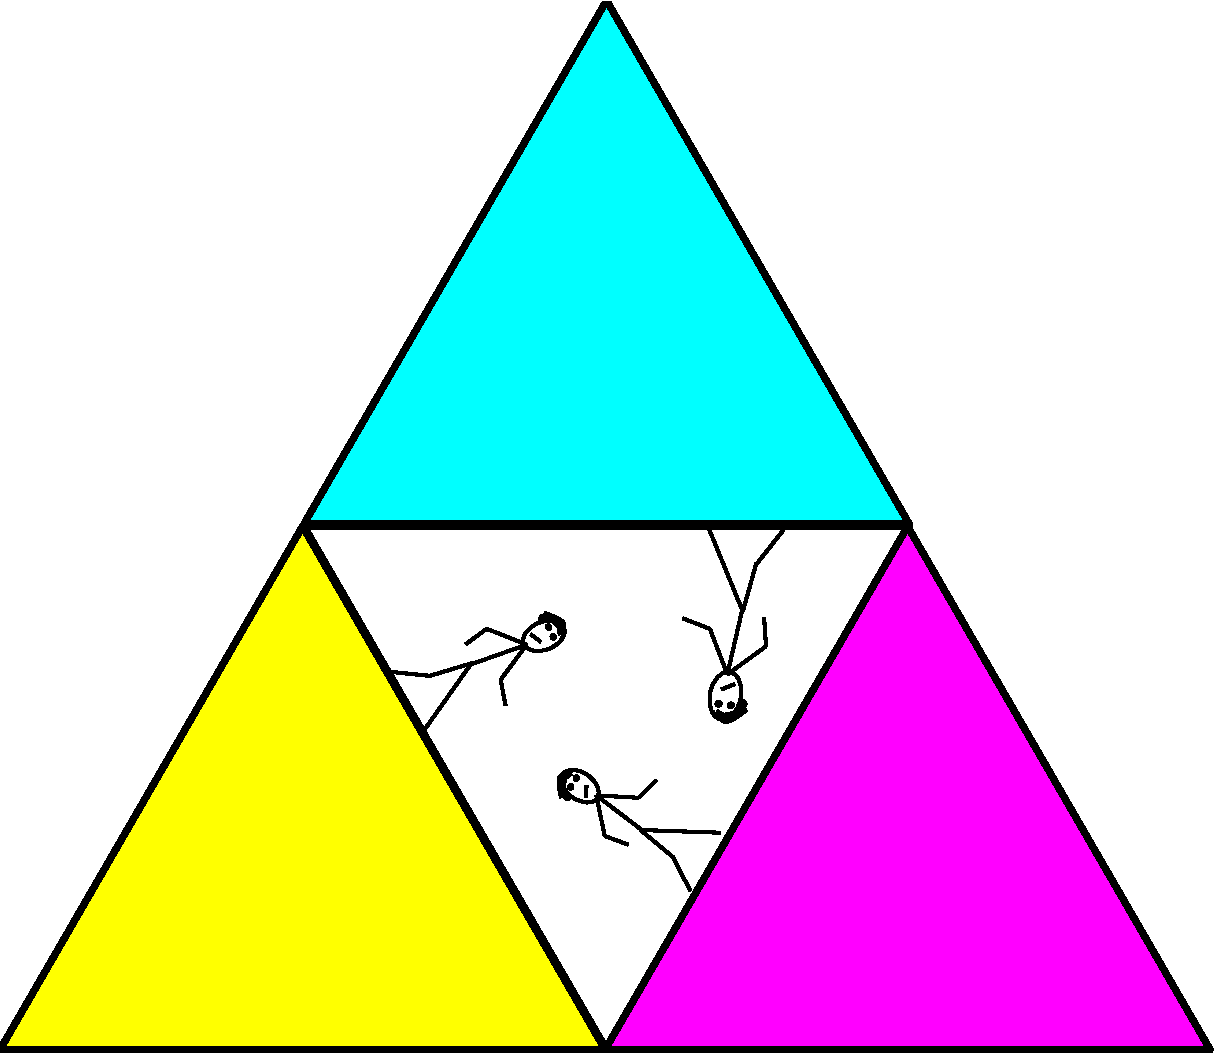
\includegraphics[width=.35\textheight]{figs/logo}
%}

\author[Bo and Raf]{{\textbf{Rafael Frongillo} and \textbf{Bo Waggoner}} \and {University of Colorado, Boulder}}
\date{\textbf{NeurIPS 2021}}

\begin{document}

%%%%%%%%%%%%%%%%%%%%%%%%%%%%%%%%%%%%%%%%%%%%%%%%%%%%%%%%%%%%%%%
\begin{frame}
  \titlepage
\end{frame}

%%%%%%%%%%%%%%%%%%%%%%%%%%%%%%%%%%%%%%%%%%%%%%%%%%%%%%%%%%%%%%
\begin{frame}{The short version}{}
  Surrogate risk minimization for supervised learning:
  \pause
  \begin{itemize}[<+->]
    \item Goal: optimize \redem{discrete ``target''} loss $\ell(r,y)$  \hintright{e.g. classification, structured predictions, \dots}  \\
          \hint{$r = $ prediction in a finite set, $y = $ label}
    \item Approach: optimize \blueem{continuous ``surrogate''} loss $L(u,y)$  \hintright{then ``link'' to target prediction $r = \psi(u)$} \\
          \hint{$u = $ prediction in $\reals^d$}
  \end{itemize}

  \only<4>{
    \centergraphics{0.8}{figs/hinge}
  }
  \pause
  \only<5>{
    \centergraphics{0.8}{figs/hinge-link}
  }
  \pause

  \vskip2em
  Question: when does (quick) \blueem{surrogate} convergence imply (quick) \redem{target} convergence?  \\
  \hint{``Surrogate regret bounds'' or ``regret transfer rates''}

  \only<7>{
    {\Large \[ \Reg_{\ell}(\psi \circ h) \leq \zeta \Big( \Reg_L(h) \Big) \] }
    \hint{Regret = ``excess risk'' over Bayes optimal}
  }

  \pause
  \pause
  \vskip2em
  This paper: \textbf{polyhedral surrogates}  \hintright{piecewise-linear and convex}
  \pause
  \begin{enumerate}[<+->]
    \item \emph{All} polyhedral surrogates have \textbf{linear} regret transfer rates!
    \item \emph{All} sufficiently ``non-polyhedral'' surrogate transfers are \textbf{quadratically slower}.
  \end{enumerate}

  \pause
  \vskip2em
  \textbf{Polyhedral:} In all cases, \blueem{surrogate regret} $\leq \epsilon$ $\implies$ \redem{target regret} $\leq O(\epsilon)$  \\

  \vskip1em
  \pause \textbf{Non-polyhedral:} There exist cases where \blueem{surrogate regret} $\leq \epsilon$ yet \redem{target regret} $\geq \Omega(\sqrt{\epsilon})$.
\end{frame}

%%%%%%%%%%%%%%%%%%%%%%%%%%%%%%%%%%%%%%%%%%%%%%%%%%%%%%%%%%%%%%
\begin{frame}{Outline}{}
  \vfill
  {\Large
    \begin{itemize}
      \item Regret transfers (``surrogate regret bounds'') \\
            \vskip1em
      \item Polyhedral losses  \\
            \vskip1em
      \item Positive results for polyhedral surrogates  \\
            \vskip1em
      \item Negative results for sufficiently non-polyhedral surrogates
    \end{itemize}
  } % end Large
  \vfill
\end{frame}

%%%%%%%%%%%%%%%%%%%%%%%%%%%%%%%%%%%%%%%%%%%%%%%%%%%%%%%%%%%%%%
\begin{frame}{}{}
  \vfill
  {\Large
    \begin{itemize}
      \item Regret transfers (``surrogate regret bounds'') \\
            \vskip1em
      \item \hint{Polyhedral losses}  \\
            \vskip1em
      \item \hint{Positive results for polyhedral surrogates}  \\
            \vskip1em
      \item \hint{Negative results for sufficiently non-polyhedral surrogates}
    \end{itemize}
  } % end Large
  \vfill
\end{frame}

%%%%%%%%%%%%%%%%%%%%%%%%%%%%%%%%%%%%%%%%%%%%%%%%%%%%%%%%%%%%%%
\begin{frame}{Supervised learning, surrogate risk minimization}{}
  \textbf{Data:} $(x,y) \in \X \times \Y$   \hintright{from distributions $\D$}

  \vskip1em
  \pause
  \textbf{Hypotheses:} $g: \X \to \R$   \hintright{example soon}

  \vskip1em
  \pause
  \redem{Discrete target loss:} $\ell: \R \times \Y \to \reals_{\geq 0}$.  \hintright{discrete: $\R$ is finite}

  \only<4>{
    \vskip1em
    Examples:
    \begin{itemize}
      \item Classification ($0-1$ loss)     \hintright{$\R = \Y$}
      \item Classification with abstention  \hintright{$\R = \Y \cup \{\bot\}$}
      \item Ranking \hintright{$\R = $ permutations of $\Y$}
      \item Top-$k$ \hintright{$\R = $ size-$k$ subsets of $\Y$}
    \end{itemize}
  } % end only

  \pause
  \pause
  \vskip1em
  \textbf{Regret:} $\Reg_{\ell}(g;\D) := \E_{x,y \sim \D} \left[ \ell(g(x), y) - \ell(g^*(x), y) \right]$.  \hintright{$g^* = $ Bayes optimal}

  \pause
  \vskip1em
  \blueem{Continuous surrogate loss:} $L: \reals^d \times \Y \to \reals_{\geq 0}$.  \hintright{for some $d$}

  \pause
  \vskip1em
  Examples:
  \begin{itemize}
    \item Hinge loss for classification ($0-1$ loss)
    \item BEP surrogate for classification with abstention  \hintright{Ramaswamy et al. 2018}
    \item ...
  \end{itemize}
\end{frame}

%%%%%%%%%%%%%%%%%%%%%%%%%%%%%%%%%%%%%%%%%%%%%%%%%%%%%%%%%%%%%%
\begin{frame}{What makes for a good \blueem{surrogate}?}{}
  \pause
  \textbf{1.} Optimizable. \\
  \hint{Convex; strongly convex, etc.}

  \pause
  \vskip1em
  \textbf{2.} Generalization bound; convergence rate. \\
  \hint{e.g. with $n$ data points, $\Reg_L(h;\D) \leq O(\sqrt{1/n})$.}

  \pause
  \vskip1em
  \textbf{3. Connection to the \redem{target}.}

  \pause
  \vskip1em
  Formalize via \textbf{regret transfer function} (also called \emph{calibration function}) $\zeta: \reals_{\geq 0} \to \reals_{\geq 0}$:  \hintright{continuous at zero, $\zeta(0) = 0$}

  \[ \Reg_{\ell}(\psi \circ h ; \D) ~ \leq ~ \zeta\Big( \Reg_L(h ; \D) \Big) . \]

  \pause
  \vskip1em
  If \textbf{any such $\zeta$} exists, $(L,\psi)$ is \textbf{consistent} for $\ell$.  \\
  \hint{As $\Reg_L(h^{(n)}; \D) \to 0$, we have $\Reg_{\ell}^{(n)}(\psi \circ h^{(n)} ; \D) \to 0$.}

  \vskip1em
  \pause
  Ideally: \textbf{fast} convergence, e.g. $\zeta(\epsilon) = O(\sqrt{\epsilon})$ (good), ~~ $O(\epsilon^{3/4})$ (better), ~~ $O(\epsilon)$ (best).

  \vskip1em
  \pause
  Prior work: binary classification (Zhang et al. 2004, etc.); bipartite ranking (Agarwal 2014, etc.); multiclass classification (Duchi et al. 2018, etc.); hierarchical classification (Ramaswamy et al. 2015); strongly convex surrogates (Nowak-Vila et al. 2019, etc.).
\end{frame}

%%%%%%%%%%%%%%%%%%%%%%%%%%%%%%%%%%%%%%%%%%%%%%%%%%%%%%%%%%%%%%
\begin{frame}{}{}
  \vfill
  {\Large
    \begin{itemize}
      \item \hint{Regret transfers (``surrogate regret bounds'')} \\
            \vskip1em
      \item Polyhedral losses  \\
            \vskip1em
      \item \hint{Positive results for polyhedral surrogates}  \\
            \vskip1em
      \item \hint{Negative results for sufficiently non-polyhedral surrogates}
    \end{itemize}
  } % end Large
  \vfill
\end{frame}

%%%%%%%%%%%%%%%%%%%%%%%%%%%%%%%%%%%%%%%%%%%%%%%%%%%%%%%%%%%%%%
\begin{frame}{Polyhedral losses}{}
  A function is \textbf{polyhedral} if it is the pointwise maximum of a finite set of affine functions.  \\
  \hint{``Piecewise-linear convex''}

  \pause
  \vskip1em
  The \blueem{surrogate loss} $L: \reals^d \times \Y \to \reals_{\geq 0}$ is \textbf{polyhedral} if each $L(\cdot ,y)$ is polyhedral.

  \pause
  \vskip1em
  Recent work: \blueem{polyhedral surrogates} are natural convexifications of \redem{discrete losses}.
  \begin{itemize}[<+->]
    \item Finocchiaro, \textbf{Frongillo}, \textbf{Waggoner} 2019:
    \begin{itemize}
      \item Every \redem{discrete loss} $\ell$ has a consistent \blueem{polyhedral surrogate} $(L,\psi)$.
      \item Further, that surrogate is obtained by ``embedding'' $\ell$ in $\reals^d$.
    \end{itemize}
    \item Finocchiaro, \textbf{Frongillo}, \textbf{Waggoner} 2020: investigates dimensionality $d$
    \item Inspiration: BEP surrogate of Ramaswamy et al. 2018
    \item Recent work, applications: Wang and Scott 2020 on Westin-Watkins hinge
  \end{itemize}
\end{frame}

%%%%%%%%%%%%%%%%%%%%%%%%%%%%%%%%%%%%%%%%%%%%%%%%%%%%%%%%%%%%%%
\begin{frame}{}{}
  \vfill
  {\Large
    \begin{itemize}
      \item \hint{Regret transfers (``surrogate regret bounds'')} \\
            \vskip1em
      \item \hint{Polyhedral losses}  \\
            \vskip1em
      \item Positive results for polyhedral surrogates  \\
            \vskip1em
      \item \hint{Negative results for sufficiently non-polyhedral surrogates}
    \end{itemize}
  } % end Large
  \vfill
\end{frame}

%%%%%%%%%%%%%%%%%%%%%%%%%%%%%%%%%%%%%%%%%%%%%%%%%%%%%%%%%%%%%%
\begin{frame}{Polyhedral surrogates guarantee linear regret transfer}{}
  \begin{theorem}
    Suppose $L$ is polyhedral and $(L,\psi)$ are consistent for the discrete target $\ell$.
    Then there exists $C > 0$ such that, for all $\D$ and $h$,
    \[ \Reg_{\ell}(\psi \circ h; \D) \leq C \cdot \Reg_L(h; \D) . \]
  \end{theorem}

  \pause
  \vskip1em
  \emph{Proof sketch.}
  Fix $x$; let $p,q \in \simplex$ be distributions of $y$ given $x$.
  \begin{itemize}[<+->]
    \item Suffices to prove that for all $p$ and $u$, $\Reg_{\ell}(\psi(u);p) \leq C \cdot \Reg_L(u;p)$.
    \item Consistent $\implies$ for all $q$, there exists $\alpha_q > 0$ such that $\Reg_{\ell}(\psi(u); q) \leq \alpha_q \cdot \Reg_L(u; q)$.
    \item Polyhedral losses have a \textbf{finite structure}: \hintright{Closely related to embeddings framework}
    \begin{itemize}
      \item There is a finite $U \subseteq \reals^d$ such that, for all $p$, $U$ contains an optimal prediction.
      \item These $U$ partition $\simplex$ into finitely many polytopes.
    \end{itemize}
    \item Regret is linear on each polytope.
    \item Therefore $\Reg_L(u ; p)$ is a convex combination over the corners.
    \item So we can take $C = \max_{\text{corners $q$}} \alpha_q$.
  \end{itemize}
\end{frame}

%%%%%%%%%%%%%%%%%%%%%%%%%%%%%%%%%%%%%%%%%%%%%%%%%%%%%%%%%%%%%%
\begin{frame}{Investigating the constant}{}
  \begin{theorem}
    Suppose $L$ is polyhedral and $(L,\psi)$ are consistent for the discrete target $\ell$.
    Then there exists $C > 0$ such that, for all $\D$ and $h$,
    \[ \Reg_{\ell}(\psi \circ h; \D) \leq C \cdot \Reg_L(h; \D) . \]
  \end{theorem}

  \pause
  \vskip1em
  $C = \max_{\text{corners $q$}} \alpha_q$.

  \pause
  \vskip1em
  What is $C$?

  \pause
  \vskip1em
  Can bound $C \leq \beta_{L} \cdot \beta_{\ell} \cdot \beta_{\psi}$.

  \pause
  \vskip1em
  \begin{itemize}
    \item $\beta_L$ comes from \textbf{Hoffman constants}.  \hintright{minimum slope of polyhedral losses}
    \item $\beta_{\ell}$ comes from a simple maximum possible regret.
    \item $\beta_{\psi} = \frac{1}{\epsilon}$ where the link is $\epsilon$-separated. \hintright{see embedding framework}
  \end{itemize}
\end{frame}

%%%%%%%%%%%%%%%%%%%%%%%%%%%%%%%%%%%%%%%%%%%%%%%%%%%%%%%%%%%%%%
\begin{frame}{}{}
  \vfill
  {\Large
    \begin{itemize}
      \item \hint{Regret transfers (``surrogate regret bounds'')} \\
            \vskip1em
      \item \hint{Polyhedral losses}  \\
            \vskip1em
      \item \hint{Positive results for polyhedral surrogates}  \\
            \vskip1em
      \item Negative results for sufficiently non-polyhedral surrogates
    \end{itemize}
  } % end Large
  \vfill
\end{frame}

%%%%%%%%%%%%%%%%%%%%%%%%%%%%%%%%%%%%%%%%%%%%%%%%%%%%%%%%%%%%%%
\begin{frame}{Non-polyhedral surrogates}{}
  \begin{theorem}
    Let $L$ be a locally strongly convex surrogate with locally Lipschitz gradient.
    Suppose $(L,\psi)$ is consistent for $\ell$ with:
    \[  \Reg_{\ell}(\psi \circ h) \leq \zeta\Big( \Reg_L(h) \Big) . \]
   Then there exists $c > 0$ such that, for all small enough $\epsilon > 0$,
    \[ \zeta(\epsilon) \geq c \sqrt{\epsilon} . \]
  \end{theorem}

  \pause
  \emph{Proof idea:}
  \begin{itemize}
    \item Fix a ``boundary'' prediction $u_0$.
    \item Consider a conditional distributions $\{p_{\lambda} : 0 \leq \lambda \leq 1\}$
    \item \redem{Target regret} shrinks linearly as $\lambda \to 0$
    \item But \blueem{Surrogate regret} shrinks with $\sqrt{\lambda}$.
  \end{itemize}

  \pause
  Example: exponential loss,  \hintright{not strongly convex, but locally s.c.}  \\
  Huber loss                  \hintright{via a strengthening of the theorem}
\end{frame}

%%%%%%%%%%%%%%%%%%%%%%%%%%%%%%%%%%%%%%%%%%%%%%%%%%%%%%%%%%%%%%
\begin{frame}{}{}
  \vfill
  {\Large
    \begin{itemize}
      \item \hint{Regret transfers (``surrogate regret bounds'')} \\
            \vskip1em
      \item \hint{Polyhedral losses}  \\
            \vskip1em
      \item \hint{Positive results for polyhedral surrogates}  \\
            \vskip1em
      \item \hint{Negative results for sufficiently non-polyhedral surrogates}  \\
            \vskip1em
      \item Conclusion
    \end{itemize}
  } % end Large
  \vfill
\end{frame}



\begin{frame}{Big picture}{}
  \blueem{Polyhedral surrogate losses} are nice:
  \begin{itemize}
    \item Consistent polyhedral surrogates always exist
    \item Embedding framework
    \item \textbf{(This work) Always satisfy linear regret transfer}  \hintright{a.k.a. calibration functions}
  \end{itemize}

  \pause
  \vskip2em
  Next questions:
  \begin{itemize}
    \item Are they good for the whole pipeline? (optimization + generalization)
    \item Applications...
    \item e.g. low-dimensional or otherwise ``nice'' polyhedral surrogates
  \end{itemize}

  \pause
  \vskip2em
  \textbf{Thanks!}
\end{frame}

%%%%%%%%%%%%%%%%%%%%%%%%%%%%%%%%%%%%%%%%%%%%%%%%%%%%%%%%%%%%%%
%%%%%%%%%%%%%%%%%%%%%%%%%%%%%%%%%%%%%%%%%%%%%%%%%%%%%%%%%%%%%%
%%%%%%%%%%%%%%%%%%%%%%%%%%%%%%%%%%%%%%%%%%%%%%%%%%%%%%%%%%%%%%
%%%%%%%%%%%%%%%%%%%%%%%%%%%%%%%%%%%%%%%%%%%%%%%%%%%%%%%%%%%%%%
%%%%%%%%%%%%%%%%%%%%%%%%%%%%%%%%%%%%%%%%%%%%%%%%%%%%%%%%%%%%%%
%%%%%%%%%%%%%%%%%%%%%%%%%%%%%%%%%%%%%%%%%%%%%%%%%%%%%%%%%%%%%%

\end{document}

